% Compile from reports/: xelatex project; bibtex project; xelatex project; xelatex project
% Sources and measured results are included by relative paths. No fabricated data.
\documentclass[sigconf,nonacm]{acmart}
\usepackage[UTF8,scheme=plain,fontset=fandol]{ctex}
\usepackage{amsmath,booktabs,graphicx}
\usepackage{xurl}
\emergencystretch=1em
\setcopyright{none}
\settopmatter{printacmref=false,printccs=false,printfolios=true}
\renewcommand{\shortauthors}{信息检索原理课程项目}
\title{面向科学声明核查的证据文献检索：\texorpdfstring{\\}{ }词项与字符排名融合的效果、成本与失败分析}
\author{信息检索原理课程项目}
\affiliation{\institution{课程实验}\country{中国}}
\acmYear{2026}
\acmConference{信息检索原理}{2026年秋季}{课程实验}
\newcommand{\BaseNDCG}{0.6596}
\newcommand{\FusionNDCG}{0.6662}
\newcommand{\BaseRecall}{0.8726}
\newcommand{\FusionRecall}{0.9303}
\newcommand{\FusionDelta}{0.0066}
\newcommand{\FusionCILow}{-0.0119}
\newcommand{\FusionCIHigh}{0.0255}
\newcommand{\BaseMs}{7.4450}
\newcommand{\FusionMs}{42.4573}

\begin{document}
\begin{abstract}
科学声明核查首先需要找到相关证据文献。严格词匹配可能因词形或表达差异漏掉证据，给后续人工核查或重排留下不完整候选。本文研究能否通过不同词汇表示的排名融合减少这种漏检，以及额外成本有多大。我们围绕 Reciprocal Rank Fusion（RRF）实现完整检索与评价流程，在 BEIR 格式的 SciFact 数据上比较 BM25、词级 TF--IDF、字符级 TF--IDF，以及固定参数、加权参数和分数归一化融合。实验使用全部 5,183 篇文献；从官方 809 个训练查询中以固定随机种子抽取 200 个开发查询，冻结参数后评价官方 300 个测试查询。BM25 的 nDCG@10 为 0.6596，BM25 与字符检索的 RRF 为 0.6662，Recall@100 从 0.8726 增至 0.9303，但融合方案需要约 5.7 倍于 BM25 的串行查询时间。配对 bootstrap 显示 nDCG 增量的 95\% 区间跨越零，因此不能据此断言融合显著优于 BM25。词级两路融合甚至略低于 BM25，表明增加检索器不自动带来收益。本系统改善的是候选证据覆盖，不执行声明真假分类。项目交付可运行代码、逐查询结果、TREC 排名、数据指纹、参数搜索记录与案例分析，使结论能够追溯到实际输出。
\end{abstract}
\keywords{信息检索, 排名融合, RRF, BM25, TF--IDF, SciFact, 可复现实验}
\maketitle

\section{问题定义与项目目标}
科学声明核查者面对一句论断时，需要先从论文集合中找到可能支持或反驳它的文献。如果检索阶段漏掉证据，即使后续核查者或分类器很强，也无法使用从未进入候选集合的文献。本项目实际处理的正是这一步候选证据漏检，而不是自动完成科学论断验证。

信息检索系统通常需要在语义相关性、词汇覆盖与计算成本之间取舍。不同的检索表示会突出不同证据：词项统计强调完整词的出现与文档长度，字符片段可以覆盖词形变化、连字符拆分和部分专业名称。实际系统经常把多个检索器的候选文档合并，再决定最终排名。这里的困难不仅是得到更多候选，还包括如何处理各检索器不相同的分数尺度，以及如何避免低质量候选挤占高质量结果。

本项目选择排名融合作为主题 X，具体任务是\textbf{给定一条英文科学论断，从科学文献摘要集合中检索能够支持或反驳该论断的候选文献}。系统不负责最终判断论断真伪，也不生成医学建议；它输出的是可能包含核查证据的文献排名。这样的任务有明确的查询、文档与相关性标注，能够直接用排序指标评价，适合检验融合方法是否改善了信息获取。

我们将 RRF 原论文\cite{cormack2009rrf}中的排名合并思想迁移到较小但真实的科学检索任务。目标是实现并检验思想，而不是重现原论文在 TREC 与 LETOR 上的全部数字。项目同时保留有利与不利结果，重点回答四个问题：第一，词级和字符级表示是否提供互补结果；第二，RRF 的固定参数是否可靠；第三，开发集调参能否转化为测试集收益；第四，检索质量变化是否足以抵偿额外时间。

我们的系统贡献是一个能够独立运行、审计和扩展的实验流程。它包含三种基础检索器、五种融合配置、训练与测试隔离、四项排序指标、逐查询差异统计以及终端检索演示。所有结果均来自项目代码的实际执行；本文不把课程实验包装为一种新的融合算法，也不把单一数据集上的观察推广为普遍规律。

\section{研究背景与方法选择}
\subsection{从单路检索到排名融合}
单个检索器会受到表示方式的约束。若查询和相关文档使用不同的词形，严格词匹配可能漏掉相关证据；若查询包含很常见的主题词，字符相似性又可能把主题相近但不回答问题的文档排在前面。一个自然方案是让不同系统提供各自的排名，再合并它们的意见。然而，不同检索器的原始分数通常不能直接相加。例如 BM25 是一组词项贡献之和，余弦相似度受到单位范数约束；二者的数值范围与查询敏感性不同。

RRF 用名次代替原始分数，从而避开跨系统分数量纲问题。它的吸引力在于实现简单、无需相关性训练即可运行，并且能够对同时被多个检索器发现的文档给予额外支持。原论文在所测集合上展示了较好的融合效果，但这不意味着任意检索器组合、任意候选截断都能得到同样结论。我们特别关注两个高度相关的词汇检索器是否会产生重复意见，以及较不同的字符表示是否能带来足够有效的新候选。

\subsection{为什么使用 SciFact}
SciFact 面向科学论断核查，提供论断、科学摘要与证据标注\cite{wadden2020scifact}。BEIR 将它整理为统一的检索评价格式\cite{thakur2021beir}。与只设计几个自造查询相比，这种数据具有公开来源、固定测试集合和独立相关性标注，能够检验系统在较多查询上的稳定性。另一方面，文献集合只有数千篇，因此可以在普通 CPU 上完整扫描稀疏向量，不依赖 GPU、远程模型接口或收费服务。

选择较小集合有意控制了工程范围，使主要变量集中在表示和融合，而不是分布式调度、近似向量索引或模型部署。代价是无法评价大规模索引的扩展性，也不能代表开放网页上的噪声分布。本文因此将结论限定为 SciFact 科学摘要检索与当前实现条件，不宣称已经解决通用混合检索问题。

\subsection{与主论文的对应关系}
本项目保留了原论文的核心 RRF 公式及常用的 $k=60$，但基础检索器、数据和候选深度与原论文不同。我们也增加开发集加权版本和分数融合对照，用于检验不依赖分数尺度究竟带来哪些实际益处。这里的加权版本属于项目扩展，不能说成原论文实验的复现结果。原论文报告的提升与本文测得的提升必须分开表述。

\section{数据、划分与防止评价泄漏}
\subsection{数据结构与规模}
实验使用 BEIR 发布的 SciFact 压缩包。文档文件 \path{corpus.jsonl} 包含 5,183 条文档，每条具有独立文档编号、标题和摘要。查询文件 \path{queries.jsonl} 提供科学论断文本，相关性文件采用三列格式：查询编号、文档编号和相关性分数。官方相关性集合分为 809 个训练查询与 300 个测试查询；本项目分别读取对应的 \path{train.tsv} 和 \path{test.tsv}。

每篇文档的索引文本由标题、一个空格和摘要连接得到。标题仅出现一次，没有人为提高标题权重，也没有额外引入作者、年份或引用网络。查询保持原始文本，不使用测试标注进行改写。三个检索器都使用相同文档文本，因此差异来自表示和排序方法，而不是偷偷给某个系统更多信息。

\subsection{开发集的构造}
项目不把测试查询拿来搜索参数。先将官方训练查询编号排序，再用随机种子 42 从中抽取 200 个编号，作为本实验的开发查询。其余 609 个训练查询在本轮实验中不参与调参或评价。这个选择减少了重复实验时间，同时提供一个固定、可检查的开发集合。全部 200 个编号被写入 \path{results/tuning.json}，而不是只记录随机种子。

索引器读取全部文档以计算词频和文档频率，属于该检索任务允许使用的无监督集合统计；它不读取测试查询的相关文档标签。开发参数选择结束并保存之后，实验程序才读取测试相关性文件。程序检查训练与测试查询编号交集为空，从控制流程和数据层面共同限制标签泄漏。查询编号与文档编号属于不同命名空间，不能只因为字符串相同就删除某篇候选文档；当前数据的两个编号集合事实上没有交集。

\subsection{数据完整性与可追溯性}
下载脚本使用官方公开链接，验证压缩包 MD5：\path{5f7d1de60b170fc8027bb7898e2efca1}。解压前检查成员目标路径是否仍位于数据目录，避免解压路径越界。已有正确数据无需重复下载。实验还为语料、查询和两个相关性文件分别计算 SHA--256，并将结果存入 \path{environment.json}。

这些指纹用于识别实验实际使用的输入，而不是证明标注完美无误。若未来数据版本发生变化，应当重新运行实验，不能继续沿用本文表格。项目不把数据本体复制进代码实现；复现者可以用下载脚本获取相同公开输入，再通过哈希确认是否一致。

\section{基础检索器}
\subsection{BM25 的实现}
文本先转为小写，使用 Unicode 词字符规则提取长度至少为二的词项。我们没有词干化、停用词表或领域词典。这样的处理相对简单，便于审查，但与特定搜索引擎的默认分析器并不相同。BM25 采用下式，其中 $f(t,d)$ 是词频，$|d|$ 是文档词数，$\overline L$ 是平均文档长度：
\begin{equation}
\mathrm{BM25}(q,d)=\sum_{t\in q}\mathrm{IDF}(t)
\frac{f(t,d)(k_1+1)}{f(t,d)+k_1(1-b+b|d|/\overline L)}.
\end{equation}
逆文档频率使用始终为正的形式：
\begin{equation}
\mathrm{IDF}(t)=\ln\left(1+\frac{N-\mathrm{df}(t)+0.5}{\mathrm{df}(t)+0.5}\right).
\end{equation}
本实验固定 $k_1=1.2$、$b=0.75$，没有在测试集上重新调整。查询中的重复词项重复贡献分数，没有再使用单独的查询词频饱和项。索引阶段预先计算每个文档词项的长度归一化权重，查询阶段用稀疏乘法累计匹配分数。这个实现是透明的词汇基线，不能称为 BEIR 官方 Elasticsearch 配置的精确复现。

\subsection{词级 TF--IDF}
词级 TF--IDF 使用与 BM25 相同的分词器。词频采用次线性变换 $1+\ln f$，IDF 使用平滑形式 $\ln((1+N)/(1+\mathrm{df}))+1$，之后对每篇文档向量做 $L_2$ 归一化。查询使用相同词表、IDF 和归一化规则。检索分数是查询向量与文档向量的内积，也就是该表示下的余弦相似度。

这个对照帮助隔离排序函数差异：BM25 与词级 TF--IDF 的基本词汇单位相同，但词频饱和、长度处理与归一化机制不同。如果二者排名高度相似，RRF 可能只是重复强化已有意见，无法明显弥补遗漏。这种现象不能简单归咎于 RRF 公式，而需要结合候选互补程度解释。

\subsection{字符级 TF--IDF}
字符检索使用 \path{char_wb} 分析器，在词边界内提取长度为 3 至 5 的字符片段；文档频率至少为 2，最多保留 100,000 个特征。它同样使用次线性词频、平滑 IDF 与 $L_2$ 归一化。这里的 ``字符'' 指英文文本的字符片段，而不是中文分字检索。

字符片段可以为缩写、连接形式或词形变化提供部分匹配，因此与完整词表示存在差异。不过，部分字符串相同不保证论断和文档在科学意义上相关。字符方法也可能过度关注很长的物种名或高频专业片段，把只共享主题的文献排得过高。我们将这种机制作为待检验解释，而不预先认定字符检索一定更好。

\section{排名融合与参数策略}
\subsection{固定参数 RRF}
对于一个文档 $d$，若第 $j$ 个检索器返回它的名次为 $r_j(d)$，则本项目采用：
\begin{equation}
S_{\mathrm{RRF}}(d)=\sum_{j:d\in L_j}\frac{1}{k+r_j(d)}.
\end{equation}
名次从 1 开始，各输入排名最多保留 100 篇文档。某篇文档没有出现在某个截断列表中时，该路贡献为零。这是面向实际 top-$n$ 结果的实现约定；它不等价于对所有文档都持有一个完整排列。融合后再取前 100 篇文档，避免把融合候选并集变大误当成固定深度召回改善。

固定参数实验统一取 $k=60$，分别融合 BM25 与词级 TF--IDF、BM25 与字符级 TF--IDF，以及全部三路。较大的 $k$ 会减弱第一名与较后名次之间的差距，从而相对强调多路共同发现的文档。举例来说，单路第一名贡献为 $1/61$，两路均排第六的文档贡献为 $2/66$，后者更高。这解释了共识可能修正某路误报，也解释了某路特别强的独有证据可能被压下去。

\subsection{开发集加权 RRF}
为检验两路质量不同的情况，我们扩展为 $S(d)=\sum_j w_j/(k+r_j(d))$。权重为非负数；无重复文档的输入排名是前提。对 BM25 与词级 TF--IDF 的组合，开发集搜索 $k\in\{10,30,60,100\}$，BM25 权重 $w\in\{0.5,1,2\}$，词级 TF--IDF 权重固定为 1。总计 12 个配置均记录开发集 nDCG@10。

参数按开发集 nDCG@10 最大值选择，若出现完全相同的值，则保留固定遍历顺序中最早的配置，因而选择过程确定。最终选中 $k=60$、BM25 权重为 2，开发集 nDCG@10 为 0.7035。本文没有看到测试结果后再扩大搜索空间，也没有用测试集选择是否报告字符路线。

\subsection{归一化分数融合对照}
排名融合不是唯一可行方案。项目还实现对两个截断结果列表分别做 min--max 归一化，再线性组合的对照：
\begin{equation}
\begin{aligned}
\widehat s_j(d)&=\frac{s_j(d)-s_{j,\min}}{s_{j,\max}-s_{j,\min}},\\
S(d)&=\alpha\widehat s_1(d)+(1-\alpha)\widehat s_2(d).
\end{aligned}
\end{equation}
未出现在该路候选中的文档贡献为零；若列表内分数完全相同，已有候选的归一化分数定义为 1。开发集搜索 $\alpha$ 分别取 0、0.25、0.5、0.75 和 1，最终选择 $\alpha=1$，开发集 nDCG@10 为 0.6996。这意味着当前两路配置下，开发集宁愿只保留 BM25 分数，也不支持等权混合。

这个端点结果具有解释价值，不能为了让 ``融合'' 显得有效而排除。本文报告的实现仍计算两个基础列表后再融合，因此即便权重为零，时间表里仍包含该路开销。工程部署可以针对端点配置跳过无用检索；本文的实测时间描述当前程序，而不是该方法的性能下界。

\subsection{核心流程伪代码}
\begin{figure}[t]
\small
\begin{tabular}{p{0.96\columnwidth}}
\toprule
\textbf{输入：}文档集合、训练相关性、查询集合；候选深度 100\\
1. 用标题和摘要构造三种无监督索引。\\
2. 固定种子从训练查询抽取 200 个开发查询。\\
3. 对开发查询计算基础排名，搜索 RRF 与分数融合参数。\\
4. 保存参数和开发查询编号，冻结选择。\\
5. 此时才读取测试相关性与 300 个测试查询编号。\\
6. 对每个测试查询检索三路候选，只保留正匹配。\\
7. 将候选名次映射为融合分数，按分数降序、文档编号升序打破平局。\\
8. 保存 TREC 排名，计算指标和逐查询差值。\\
9. 用配对 bootstrap 汇总差值的不确定性。\\
\textbf{输出：}排名、指标、开发记录、环境、案例及图表。\\
\bottomrule
\end{tabular}
\caption{项目的检索、调参与评价流程。标签隔离是程序顺序的一部分。}
\label{fig:workflow}
\end{figure}

\section{评价指标与统计协议}
\subsection{排序质量}
项目报告 nDCG@10、MAP@100、MRR@10 和 Recall@100。所有查询使用相同的宏平均权重，未标注文档按不相关处理。nDCG 的收益直接使用相关性标注值，与 \path{trec_eval} 的 \path{ndcg_cut} 定义一致：
\begin{equation}
\begin{aligned}
\mathrm{DCG}@10&=\sum_{i=1}^{10}\frac{\mathrm{rel}(d_i)}{\log_2(i+1)},\\
\mathrm{nDCG}@10&=\frac{\mathrm{DCG}@10}{\mathrm{IDCG}@10}.
\end{aligned}
\end{equation}
SciFact 本实验使用的相关性为二值。nDCG 强调用户先看到的十篇文档，并允许相关文档数量不相同的查询进行比较。MRR@10 取前十位首个相关文档名次的倒数，若前十位没有相关文档则为零，反映找到第一份证据的难易程度。

设查询相关文档集合为 $R_q$，前 $i$ 位精度为 $P_q(i)$，平均精度为：
\begin{equation}
\mathrm{AP}_q@100=\frac{1}{|R_q|}\sum_{i=1}^{100}P_q(i)\,\mathbb I[d_i\in R_q].
\end{equation}
MAP 是 AP 在查询上的平均。注意分母是\emph{全部相关文档数}，而不是检索到的相关文档数，也不是为了提高结果而缩小的分母。Recall@100 则是前一百篇结果中的相关文档数除以 $|R_q|$。这两个指标有助于区分 ``前面排得好'' 与 ``候选证据找得全''。

评价程序对无相关文档查询和空结果列表明确定义零值，避免除零或静默丢弃查询。数据文件和实验输出均保留查询编号，所以既能检查总体均值，也能追踪单条查询。只报告平均值会隐藏严重失败，本项目因此另外输出逐查询指标和正反案例。

\subsection{配对 bootstrap}
比较某种融合方法与 BM25 时，我们先为每个测试查询计算 nDCG@10 差值 $\Delta_q$。使用随机种子 42，从这 300 个差值中有放回抽取 300 个，求样本均值，重复 2,000 次。均值分布的 2.5 与 97.5 百分位构成本文的 95\% 百分位 bootstrap 区间。

配对重采样使同一个查询在两个方法下对应，避免把查询难度差异误当成方法差异。这里的区间用于描述当前测试集合上平均差值的不确定性；它并不能解决数据领域偏差，也不能证明对所有未来查询有效。我们同时报告胜、平、负查询数，帮助理解均值是来自少量大幅变化还是广泛改善。由于比较了多种配置，本文不依据这些区间进一步宣称跨方法的严格最优性。

\subsection{计时协议}
计时使用 Python 单调高精度计时器，索引构建与查询阶段分开。每个基础检索器先运行一次查询预热，预热不进入统计；随后对每个测试查询记录文本向量化、打分、排序与截断的总时间。平均值和第 95 百分位都写入输出。本实验没有多请求并发，也没有用多线程流水线隐藏慢检索器。

融合的查询时间为所需各基础查询的分别实测时间之和，加上融合本身的实测时间。这是显式串行执行的成本估计，不是把多路并行运行后的墙钟时间。比较相同输入与当前代码能够说明成本来源，但操作系统调度、CPU 频率和缓存状态会影响毫秒数，因此跨机器复现时应重点核对质量指标及数量级，不能要求时间逐位相同。

\section{实验环境与实现检查}
实验在 Windows 11 的 CPU 环境执行，Python 版本为 3.12.14，NumPy 为 2.2.6、SciPy 为 1.15.3、scikit-learn 为 1.6.1。处理器报告为 Intel64 Family 6 Model 151。全部检索器使用 SciPy 稀疏矩阵运算；不需要神经网络模型或 GPU。依赖安装在项目独立虚拟环境内，避免把可复现性建立在用户机器上偶然存在的库版本之上。

基础排序器仅输出分数严格大于零的匹配。若查询完全不在词表中，不补入若干分数为零的任意文档来凑足一百条。所有分数相同的候选按文档编号的字典序稳定排序，输入列表包含重复文档时 RRF 主动报错。稳定排序不会消除平局本身，但能避免不同机器上的容器顺序改变结果。编号只是确定规则，不是相关性信号。

项目的单元测试包括可手算的 nDCG、AP、MRR 与 Recall；空结果和零相关性；RRF 对称平局和权重；重复文档拒绝；基本词汇检索和零匹配；以及相关文档总数超过截断深度时的 AP 分母检查。六项测试全部通过。我们还使用独立验证脚本从八份 TREC 文件重建排名，在全部 300 查询上重新计算四项指标，逐项与保存的 JSON 比较，差异低于 $10^{-12}$。

这些验证并不意味着实现没有任何优化空间。它们主要覆盖最容易使结论失真的边界：把未召回的文档当成已召回、错误的 AP 分母、平局不确定性，以及报告表格与实际排名不一致。全文数字由机器结果生成的 LaTeX 表格导入，减少人工抄写造成的数据漂移。

\section{总体实验结果}
\begin{table*}[t]
\centering
\begin{tabular}{lrrrrr}
\toprule
Method & nDCG@10 & MAP@100 & MRR@10 & R@100 & ms/query \\
\midrule
BM25 & 0.6596 & 0.6197 & 0.6250 & 0.8726 & 7.45 \\
Word TF--IDF & 0.6286 & 0.5827 & 0.5897 & 0.8916 & 7.32 \\
Char TF--IDF & 0.6547 & 0.5975 & 0.6034 & 0.9187 & 34.85 \\
RRF word ($k=60$) & 0.6574 & 0.6126 & 0.6195 & 0.8882 & 14.92 \\
RRF char ($k=60$) & 0.6662 & 0.6217 & 0.6253 & 0.9303 & 42.46 \\
RRF all ($k=60$) & 0.6637 & 0.6146 & 0.6201 & 0.9259 & 49.83 \\
Weighted RRF (dev) & 0.6602 & 0.6193 & 0.6243 & 0.8726 & 14.92 \\
Score fusion (dev) & 0.6596 & 0.6197 & 0.6250 & 0.8726 & 14.88 \\
\bottomrule
\end{tabular}

\caption{SciFact 官方 300 个测试查询的结果。所有输入候选深度均为 100。Word 表示词级 TF--IDF，Char 表示字符级 TF--IDF；dev 表示只用开发集选定参数。查询时间含串行基础检索及融合，不含索引构建。}
\label{tab:results}
\end{table*}
表~\ref{tab:results} 汇总八种方法。BM25 的 nDCG@10 为 0.6596，是两种词级方法中较强的一种；词级 TF--IDF 为 0.6286。字符级 TF--IDF 的 nDCG@10 为 0.6547，与 BM25 接近，但 Recall@100 为 0.9187，明显高于 BM25 的 0.8726。这说明不同表示的主要差异不只体现在前几名，还体现在候选集合覆盖。

固定参数 BM25 与词级 TF--IDF 的 RRF 得到 0.6574，略低于 BM25；它的 Recall@100 为 0.8882，说明增加候选覆盖并没有必然改进前十排序。BM25 与字符级 TF--IDF 的 RRF 得到本表较高的 nDCG@10，数值为 0.6662，Recall@100 为 0.9303。不过，这个结果只能称为\emph{本次评价中均值较高}，还需要结合不确定性检验解读。

三路 RRF 的 nDCG@10 为 0.6637，低于 BM25 与字符的两路融合。增加一个词级列表没有进一步改善排序，可能因为它与 BM25 的判断较相似，却仍能改变共识权重。这种解释与表示机制相符，但本实验没有直接测量排名相关系数，因此不能当作已经得到严格因果证明的结论。更可靠的结论是：在固定候选深度与等权配置下，更多输入列表不是单调收益。

开发集选中的加权词级 RRF 为 0.6602，相比固定等权版本有所恢复，但对 BM25 的提升仅约 0.0006。开发集选择的分数融合参数完全退化为 BM25，测试结果与 BM25 相同。这两项结果说明开发集可以避免一部分不合适的等权组合，却不能保证得到有实际意义的新收益。调参的成功与否应由独立测试决定，而不是只引用开发集的最大值。

\subsection{召回提升与前排收益的区别}
RRF-char 的 Recall@100 相比 BM25 增加约 0.0578，即 5.78 个百分点；nDCG@10 仅增加约 0.0066。这个差异说明，新增相关文档并不总是出现在用户最先看到的位置。如果系统后面还有更强的重排器，较高候选召回可能有用；如果直接把前十篇展示给用户，那么较高延迟换来的收益则较有限。本文没有实现额外重排器，因此不能把潜在后续收益写成已经实现的结果。

此外，SciFact 中一个查询往往只有少量已标注证据，候选中找到或漏掉一篇就可能明显改变 Recall。我们采用宏平均，确保难查询没有被大量容易查询的文档数淹没，但这种指标仍会受到不完整标注影响。新增未标注文档被视为不相关，不等于它们一定没有科学价值；本文只对公开检索标注上的表现负责。

\subsection{不确定性与查询级分布}
相对于 BM25，RRF-char 的 nDCG@10 平均差值为 0.00657，95\% bootstrap 区间约为 $[-0.01193,0.02555]$。该区间跨越零，无法据此排除均值提升来自当前查询抽样差异的可能性。测试查询中有 49 个改善、217 个不变、34 个退步。多数查询没有变化，少量查询的升降共同决定了总体均值。

词级 RRF 的差值为 $-0.00226$，区间约为 $[-0.01337,0.00815]$；三路 RRF 的差值为 0.00409，区间也跨零。加权词级 RRF 的区间约为 $[-0.00326,0.00460]$。因此，我们将本项目结论表述为\textbf{融合提供了可观察的互补候选与成本变化，但在此测试集上没有获得 nDCG@10 的明确显著提升证据}。这比只选最好均值展示更符合实际实验结果。

\begin{figure}[t]
\centering
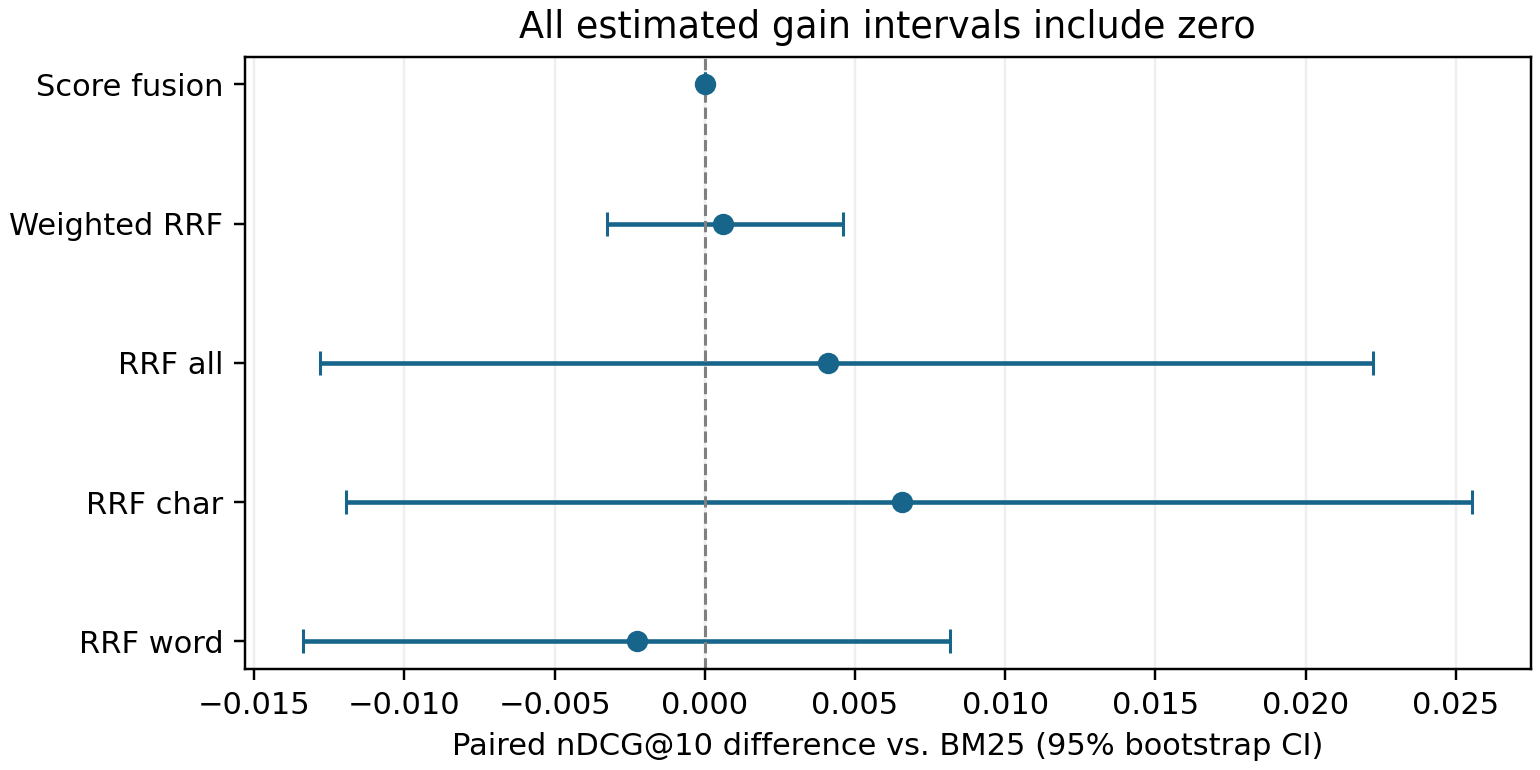
\includegraphics[width=\columnwidth]{../results/figures/bootstrap_delta.png}
\caption{各融合方法相对 BM25 的配对 nDCG@10 差值及 95\% bootstrap 区间。所有区间包含零。}
\label{fig:bootstrap}
\end{figure}

\section{效率与质量成本分析}
BM25 索引构建约需 0.487 秒，词级 TF--IDF 约需 0.479 秒，字符级 TF--IDF 约需 13.083 秒。字符路线需要提取更多片段、统计更大的特征空间，其构建时间明显较高。这一成本可在离线阶段摊销，但如果文档频繁更新，重建开销就不能忽略。本文没有实现在线增量索引，因此只报告一次完整构建的结果。

平均基础查询时间分别约为 BM25 7.45 毫秒、词级 TF--IDF 7.32 毫秒、字符级 TF--IDF 34.85 毫秒。BM25 与字符的 RRF 平均约为 42.46 毫秒，约为 BM25 的 5.70 倍；三路融合约为 49.83 毫秒。融合公式自身很轻，主要成本来自多路候选生成，尤其是字符向量的稀疏匹配。将 RRF 描述为 ``几乎免费'' 会混淆融合步骤与整条查询链路。

表中时间不代表性能充分优化后的产品系统。我们使用 Python 排序和稀疏矩阵运算，没有近似检索、倒排跳跃、向量批处理或多路并行。即便如此，相同环境下的相对成本仍能提醒设计者：当质量增量小于一个百分点、置信区间又跨零时，是否值得启用慢路线应取决于服务目标。如果任务重视候选覆盖，可优先考虑字符融合；若要求快速返回第一篇证据，BM25 已是很有竞争力的基线。

更合适的工程决策可能是按查询选择路线，而不是对所有查询无差别融合。例如完整词匹配已经给出清楚证据时，可以跳过字符检索；当查询包含连接词形、拼写变体或词表外片段时，再触发第二路。这是由结果产生的后续假设，本文尚未训练路由器或验证它的节省比例，所以不报告任何不存在的加速数字。

\begin{figure}[t]
\centering
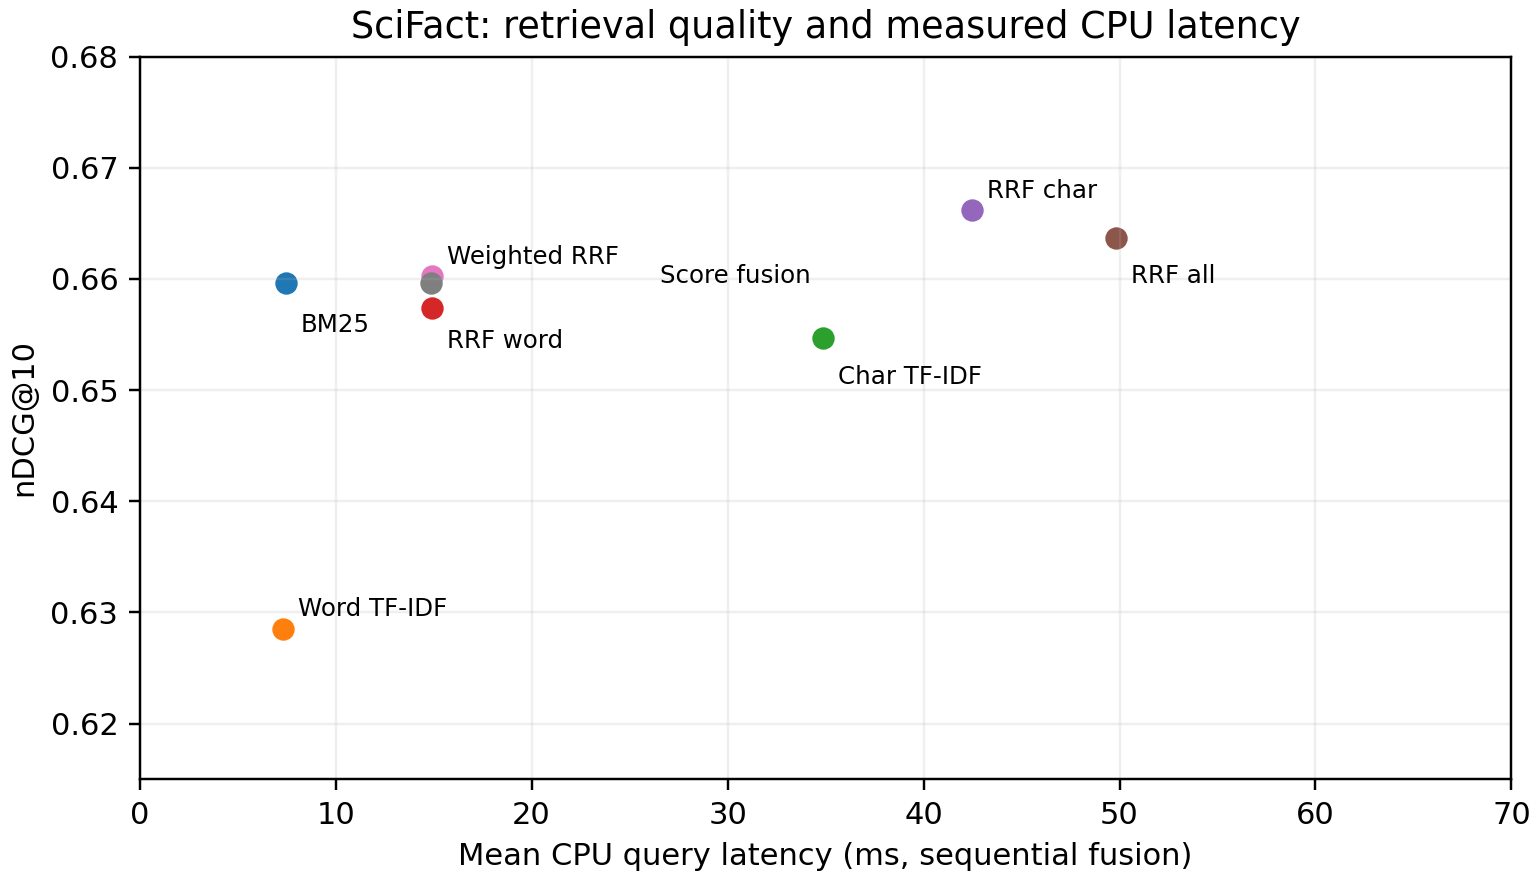
\includegraphics[width=\columnwidth]{../results/figures/quality_latency.png}
\caption{测试集质量与串行 CPU 查询时间。字符路线提高覆盖的同时，也引入主要的额外成本。}
\label{fig:latency}
\end{figure}

\section{成功与失败案例}
\subsection{案例选取方式}
为避免只展示能够支持预设结论的查询，验证脚本按 RRF-char 相对 BM25 的 nDCG@10 差值排序，分别导出最大改善与最大退步的三个查询。每个案例包含原始查询、相关文档编号和标题，以及 BM25、字符检索与融合的前五名结果。案例只是解释机制的线索，不作为总体效果的替代证据；下面选择其中两个较容易说明现象的例子。

\subsection{改善案例：连接形式与局部字符串}
查询 72 的文本为 ``Activator-inhibitor pairs are provided dorsally by Admpchordin.''。相关文档编号为 6076903，标题是 ``Regulation of ADMP and BMP2/4/7 at Opposite Embryonic Poles Generates a Self-Regulating Morphogenetic Field''。BM25 的 nDCG@10 为 0.3333，而 RRF-char 为 1.0000，相关文档在融合结果中上升到第一位。

这个查询含有连接形式 ``Admpchordin''，与标题中的 ``ADMP'' 不是完全相同的词项。字符片段在这种情况下有机会提供部分匹配，和完整词检索形成互补。需要强调的是，题目中含有某段相似字符串并不能单独证明全部改进都由这一因素造成；严格验证还需要移除特定片段或对照分词的消融实验。当前案例支持的是一个合理机制解释，而不是对词形处理效果的普遍承诺。

另一个改善查询 784 涉及 microRNA 对神经干细胞分化与增殖的调控。相关文献编号 2356950，BM25 的 nDCG@10 为 0.5，融合为 1.0。这提示互补收益也可能体现在多个相关概念的组合，而不仅是明显的连接词形。本文保留完整原始排名供检查，不把个别案例推导成领域语义理解能力；三种基础方法仍是词汇匹配系统。

\subsection{失败案例：共识压低独有证据}
查询 294 的论断涉及酿酒酵母基因启动子内是否存在 crossover hot spots。相关文献编号 10874408，标题为 ``Mapping Meiotic Single-Strand DNA Reveals a New Landscape of DNA Double-Strand Breaks in Saccharomyces cerevisiae''。BM25 将它排在第一位，nDCG@10 为 1.0；RRF-char 的前十位却没有该文档，nDCG@10 降为零。

观察字符检索的前排，会发现多篇结果都包含物种名称 ``Saccharomyces cerevisiae''，但主题分别涉及葡萄糖抑制、寿命或损伤响应。这些文献与论断共享明显的字符串，却不一定回答 crossover hot spots 的问题。它们如果也获得 BM25 的中等支持，RRF 的多路累计就可能超过只被某一路极高排名支持的真正证据。

这个失败与 RRF 的定义一致：它只知道名次，不知道某路第一名比第二名强多少，也不知道不同列表的错误是否相关。BM25 相关文档的高原始分数在转换为 $1/(60+r)$ 后被压缩，其他文档通过共识累加反而上升。因此，分数尺度鲁棒性与置信度丢失是同一设计的两面。若只讨论 RRF 无需归一化的优点而不讨论信息损失，就无法解释这种严重退步。

\subsection{从案例返回整体结论}
正反案例共同说明，融合的收益依赖候选之间的互补质量，而不只依赖差异有多大。两个检索器完全一致时难以增加信息；差异很大却充满误匹配时，又可能损害强基线。一个后续方向是用开发集估计查询级可靠性，或者让已有高置信候选保留更多影响力。不过，这需要额外设计与独立评价，本项目的已完成结果只支持其作为后续研究问题。

\section{复现步骤与交付物}
代码不依赖私人账号、访问令牌或远程推理服务。复现者在仓库根目录建立 Python 虚拟环境，安装 \path{requirements.txt} 中的依赖，运行下载脚本获取公开数据，再执行实验脚本。核心命令如下；在 Windows 环境中可将 \path{python} 替换为虚拟环境解释器的完整路径。
\begin{quote}\small
\path{python scripts/download_data.py}\\
\path{python -m unittest discover -s tests -v}\\
\path{python scripts/run_experiment.py}\\
\path{python scripts/verify_results.py}\\
\path{python scripts/export_report_assets.py}
\end{quote}
交互演示可运行 \path{python scripts/search.py} 并传入一条英文查询。演示默认构建 BM25 和词级 TF--IDF 索引，用 $k=60$ 的 RRF 输出文档编号、标题和摘要片段。它展示完整检索功能，但不是实验表中效果较高的字符融合配置；这样设计是为了让首次演示不必等待字符索引构建。两者不能在汇报时混淆。

\path{metrics.json} 与 \path{metrics.csv} 保存汇总数值，\path{per_query.csv} 保存逐查询指标和查询时间，每种方法的 \path{.trec} 文件保存完整前一百名排名。\path{tuning.json} 记录开发编号、所有参数候选及最终选择，\path{paired_bootstrap.json} 记录置信区间和胜平负。\path{environment.json} 记录依赖、数据规模、索引时间和哈希；\path{case_studies.json} 保存正反案例。

报告表格通过 \path{generated_metrics.tex} 导入，部分常用数字通过 \path{generated_summary.tex} 定义宏，科学图由结果 JSON 自动生成。编译报告时，应从 \path{reports} 目录执行 XeLaTeX、BibTeX，并再次执行两遍 XeLaTeX。正文使用 ACM \path{sigconf} 双栏文档类，中文由 \path{ctex} 的 Fandol 字体支持。

\section{局限性与可继续开展的实验}
首先，实验只包含一个科学摘要集合，只有三百个测试查询。结果不足以说明方法在网页、法律、代码或中文检索上同样有效。较小集合也使完整稀疏扫描能够在几十毫秒内完成，无法代表百万级文档场景。若扩展到其他 BEIR 数据集，应固定同一开发协议，并重新评价，而不是沿用本数据集的最优参数。

其次，基础方法都是稀疏词汇表示，没有神经稠密检索器或交叉编码重排器。因此本文讨论的是异构\emph{稀疏}检索的融合，不能把结果称为 BM25 与语义向量的混合检索性能。采用这种范围降低了依赖和资源需求，也使各种结果的原因相对可解释；但它不能回答神经检索器与 BM25 是否更互补。

第三，当前只固定候选深度一百，没有全面搜索深度与融合参数的相互作用。候选过浅可能漏掉某路的重要证据，过深又可能扩大弱共识的影响。由于每条候选列表截断，min--max 归一化的最小值也随深度变化。未来应在开发集上设置少量预注册深度，报告完整质量与成本曲线，避免事后挑选最有利截断。

第四，时间只来自一次机器环境中的顺序批次，虽然排除了索引和预热，却没有多次独立进程重复、性能隔离或并发负载。其精确毫秒数不适合当作部署承诺。未来可以增加多轮随机查询顺序、记录 CPU 和内存占用，再测多路并行后的实际墙钟时间。缓存、批处理和异步调度都可能改变效率比较，但不会自动改变离线排名指标。

第五，本轮开发集只搜索词级两路的权重，没有为字符两路单独调参。我们选择把固定字符融合当作预先设定的补充比较，而不是根据测试提升追加搜索。这降低了过拟合风险，也限制了字符路线的最佳可能表现。若以后探索查询路由、质量估计或权重预测，需要重新划定开发任务并保留独立测试，不能继续反复使用当前测试标签迭代。

最后，bootstrap 区间是描述性估计，样本量有限且存在多方法比较。本文没有将 ``区间包括零'' 解释为两种方法完全相同，也没有把略高均值解释成已证明优越。实验最重要的实际收获是识别了三件事：字符表示确实能补充不同候选；这种补充也会制造严重个例失败；在当前 CPU 实现中，候选生成成本远大于排名融合公式自身。后续优化应该围绕这些可测量现象展开。

\section{结论}
本项目实现了面向科学声明核查的证据文献检索系统，实际改善目标是减少 BM25 候选阶段的证据漏检。BM25 与字符 TF--IDF 的融合在本次测试中将平均 Recall@100 从 87.26\% 提高到 93.03\%，为后续人工核查或重排提供了覆盖更全的候选。然而，前十排序的 nDCG 增量置信区间跨零，串行查询时间约增加至 5.7 倍；系统也没有执行证据推理或真假分类。词级两路与三路结果表明，输入列表增加并不保证排序质量提高；开发集调参还可能合理地选择退化为单路系统。

因此，适合本项目的结论不是 ``RRF 总能战胜单个检索器''，而是\textbf{排名融合是一种容易实现、便于组合的检索工具，其价值必须通过候选互补性、独立评价和完整成本核算来判断}。代码、数据校验、参数记录、逐查询输出与报告生成链路共同构成可审阅交付物，也为后续扩展到查询级选择、稠密检索融合或重排提供了清楚的基线。

\bibliographystyle{ACM-Reference-Format}
\bibliography{references}
\end{document}
